\documentclass{article}
\usepackage{fullpage}
\usepackage{color}
\usepackage[affil-it]{authblk}
\usepackage{amsmath}
\usepackage{graphicx}
\usepackage{float}
\begin{document}
\author{Jayanth Kumar N}
\affil{Indian Institute of Science Education and Research, Pune}
\title{\textbf{Compartmental models on networks}}
\maketitle

\begin{abstract}
   In this artice we try to figure out the realtion between the total
   $R_{0}$ of a country and the $R_{0}$ of the individual cities how
   it varies with respect to migration between the cities. We model
   this using SIR and SEIR not graphs with vertices as cities and
   edges representing the migration. We try to figure out this
   relationship using numerically and analytically. To proceed
   numerically we use simulations to create data and calculate $R_{0}$
   using the relation derived here. Analytically we try to use next
   generation operator method to figure out the combined $R_{0}$
\end{abstract}

\section{Motivation}
$H_{1}N_{1}$ commonly called Swine Flu is a human respiratory
infection caused by an influenza strain, which nearly costs 284000
lives in 2009 alone globally. In \textit{epidemiology} each disease
can be modelled using compartmental models, one such commonly used
models are SIR and SEIR models. Each disease can be given a
charateristic value $R_{0}$ known as basic reproductive number which
represents the average number of infections an infected individual can
cause over its infectious period in an uninfected population. A paper
by Jesan,Menon and Sinha use the incidence data to calaculate the
$R_{0}$ of swine flu in India assuming the SIR model.
\begin{figure}[h]
  \centering
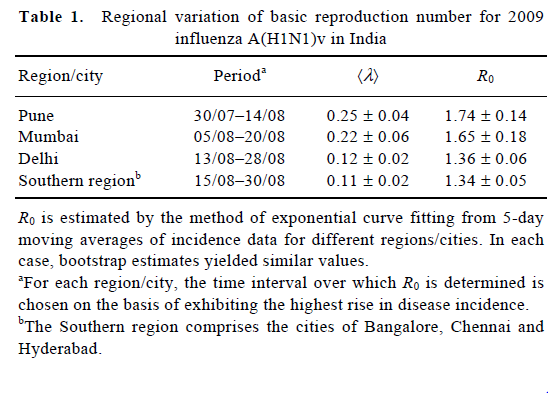
\includegraphics[scale=0.5]{table1}
\end{figure}
We see that in the table from their paper that the $R_{0}$ of India
which was calculated to be 1.45 is not the average of the $R_{0}$ of
the individual cities. So here in this article we try to find out this
relation between the $R_{0}$ of the cities and the total $R_{0}$.

\section{Methodology followed}
In order to numerically figure out the relationship between total and
individual city $R_{0}$, We try to model this scenario into simple
case with just two vertices having 3 or 4 compartments each and 2
edges represting the migration between the cities. We write down the
differential equations for these systems, which are elaborately
mentioned in the next section. We then apply Gillespie Algorithm on
these equations to stochastically simulate the models. Using this data
we try to figure out $R_{0}$ via the realtion between
intrinsic/exponential growth rate of the infected individuals and
$R_{0}$. This relation between intrinsic growth rate $r$ and $R_{0}$
depends upon the model used, we will derive the relation between them
in each case in the following sections. We will then try to see how
the total $R_{0}$ of the system change from individual $R_{0}$ of the
cities as the transfer rates between the cities are increased.  We
will try to apply the above method on SIR and SEIR(with the
restriction that the infected individuals are not allowed to migrate).
Analyically we will try to use next generation operator method on the
system of equation to derive the total $R_{0}$ of the system in the
last part of this article.
\section{Modelling using SIR model}
\begin{figure}[h]
  \centering
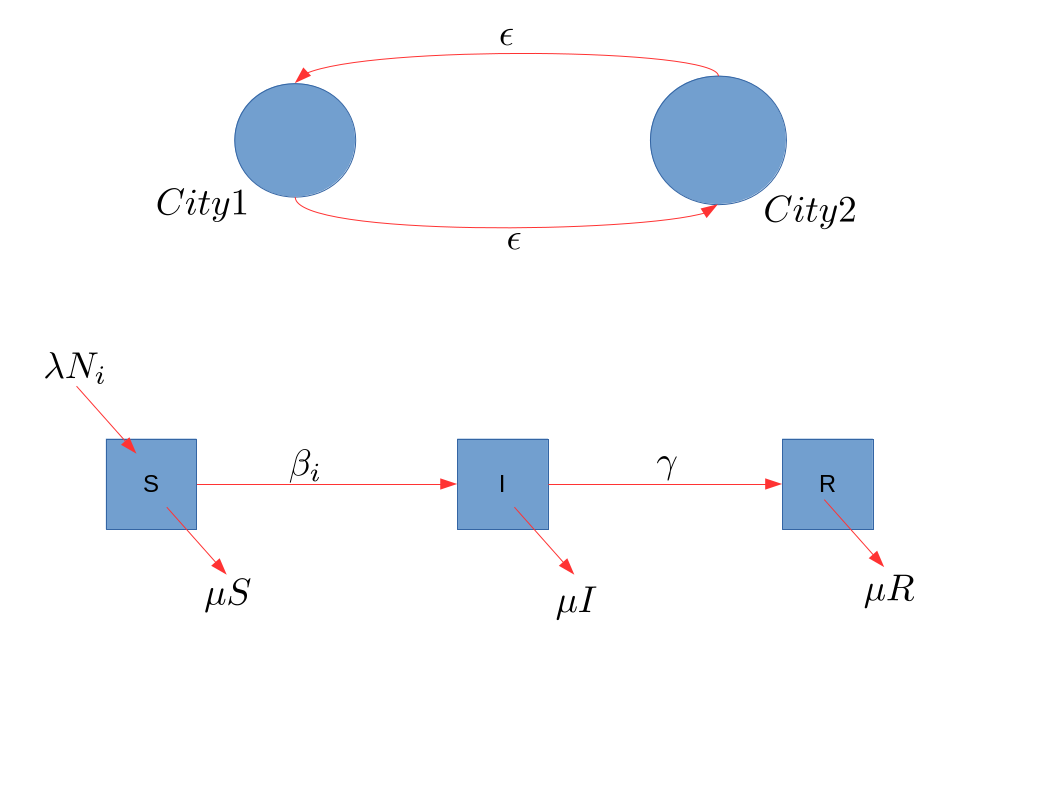
\includegraphics[scale=0.35]{sir_im}
\end{figure}
\textbf{Equations} \newline
$$\frac{dS_{1}}{dt}=\lambda(S_{1}+I_{1}+R_{1}) -\mu  S_{1} - \beta_{1} S_{1}I_{1}  + \epsilon S_{2} -\epsilon S_{1} $$  
$$\frac{dI_{1}}{dt}= -\mu  I_{1} + \beta_{1} S_{1}I_{1}  + \epsilon I_{2} -\epsilon I_{1} -\gamma I_{1} $$ 
$$\frac{dR_{1}}{dt}= -\mu  R_{1} +  \epsilon R_{2} -\epsilon R_{1} +\gamma I_{1} $$ 
$$\frac{dS_{2}}{dt}=\lambda(S_{2}+I_{2}+R_{2}) -\mu  S_{2} - \beta_{2} S_{2}I_{2}  + \epsilon S_{1} -\epsilon S_{2} $$  
$$\frac{dI_{2}}{dt}= -\mu  I_{2} + \beta_{2} S_{2}I_{2}  + \epsilon I_{1} -\epsilon I_{2} -\gamma I_{2} $$ 
$$\frac{dR_{2}}{dt}= -\mu  R_{2} +  \epsilon R_{1} -\epsilon R_{2} +\gamma I_{2} $$ 

where $\lambda$ is the birth rate,$\mu$ is the death rate,$\gamma$ is
the recovery rate and $\beta_{i}$ is the contact rate in city i. \newline

The above model was stochastically simulated using Gillespe
algoritm. Below is the graph of one such simulation.
\begin{figure}[h]
  \centering
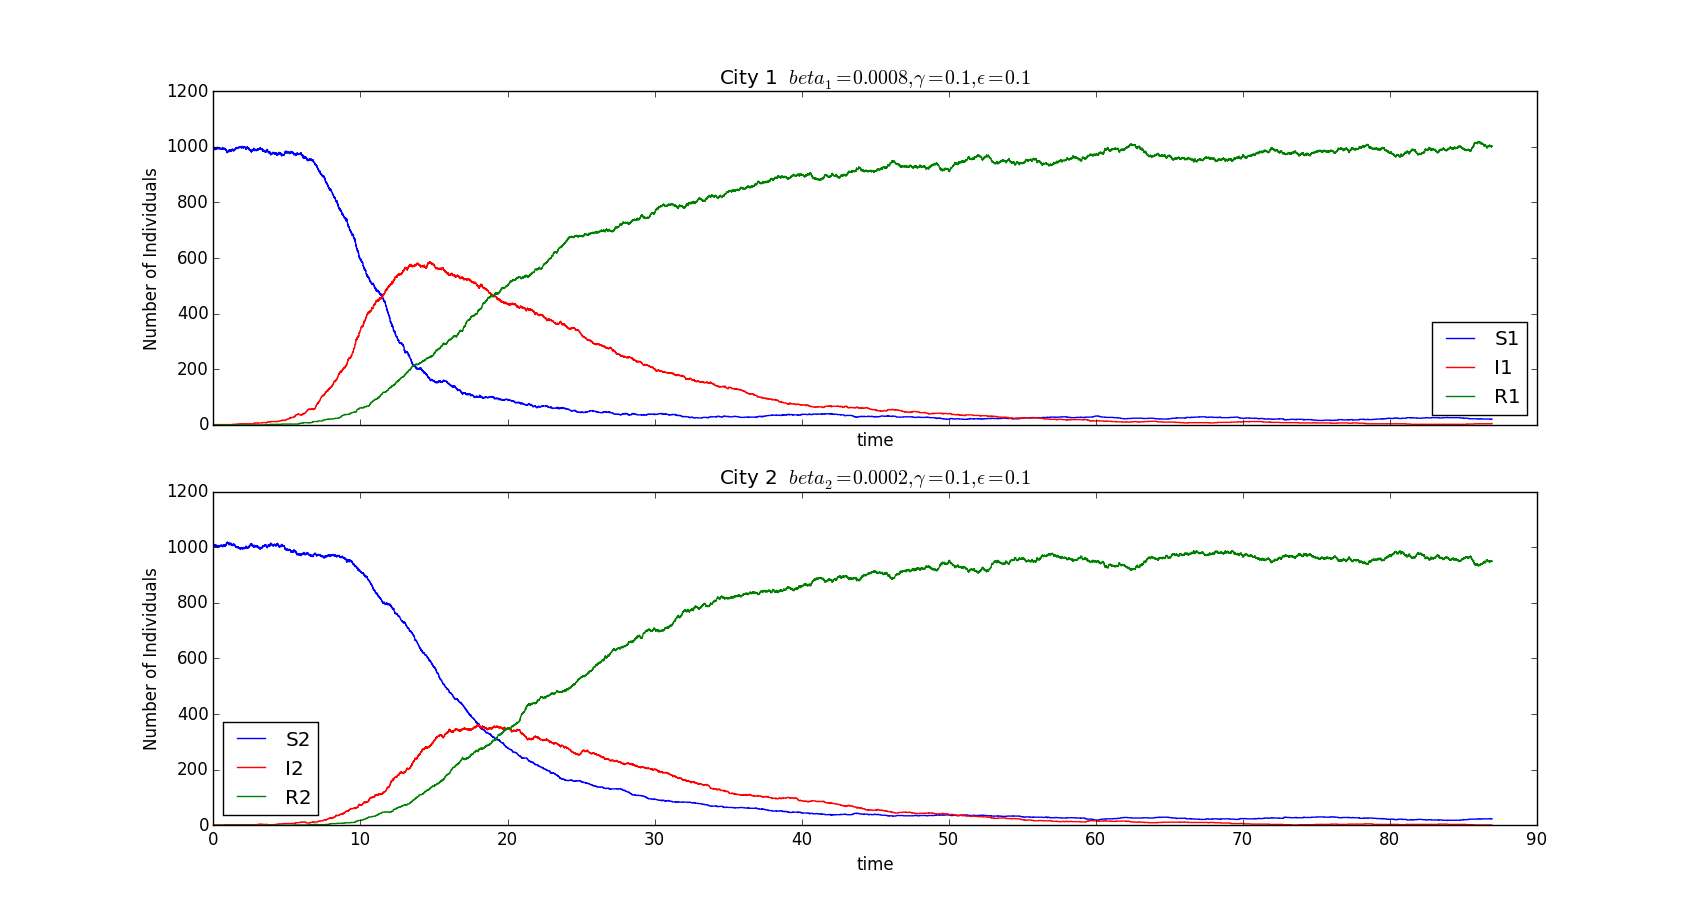
\includegraphics[width=\textwidth]{Stochstic_sim}
\end{figure}

Using this simulation we can obtain the time series of the infected
individuals in each city and for the system(by adding the individual
time series). We now try to figure out the relation between the
intrinsic growth rate $r$ and $R_{0}$. At initial conditions when
$S_{i}=N_{i}$ and $I=0$, $$\frac{dI}{dt}=rI$$
integrating, $$I(t)=ce^{rt}$$ where $c$ is a constant. Hence to
calculate $r$ we can fit a straight line to $log(I)$ vs $t$ at inital
part and the slope of this line should give $r$.
\subsection{Relation between $r$ and $R_{0}$}
We start by deriving \textbf{Lotka-Euler} equation and then applying epidemology to it.\newline
\textbf{Assumptions} 
\begin{enumerate}
\item There are only females in the population and can reproduce independent of males.
\item time and age are measured in years. $t=0$ denotes the present time
\item The population displays exponential growth rate at a fixed growth rate
\item Age distribution of the population does not change with time.
\end{enumerate}
\begin{itemize}
  \item Total No. of births at time $t$ = $\sum$ all children born to
    \textbf{all ages of mothers} at a particular time $t$.
  \item No. of births to mother of age $a$ at time $t$ = (Total number of births at time $t-a$)$\times$(Expected No. of offsprings per year for mother of age $a$)
\end{itemize}
\textbf{Note:}(Total number of births at time $t-a$) denotes the total
number of mother of age $a$ at time $t$, ie these many were born. \newline
Combining above two equations we get,
$$b(t)=\int_{a=0}^{\infty}b(t)n(a)da$$ where $b(t)$ denotes the number
of birth at time $t$ and $n(a)$ denotes the expected number of offsprings a
single mother of age $a$ will produce. \newline Since population is
growing exponentially with a constant exponential rate $r$,\newline
No. of birth at time $t$ = (No. of births at time
$t-a$)$\times$(Exponential growth from time $a$)
$$b(t)=b(t-a)e^{ra}$$
From above equations we get
\begin{equation}
b(t)=\int_{a=0}^{\infty}b(t)e^{-ra}n(a)da
\end{equation}
Define $R$ as
$R=\int_{a=0}^{\infty}n(a)da$ total number of offsprings a single
women will produce in her lifetime.\newline Define $g(a)$ as
$\frac{n(a)}{R}$ this will denote the probability that a female will
produce an offspring at age $a$, which is the PDF of the female
producing the offspring over her life time.  Now we relate this to
epidemology by considering birth of offspring=production of new
infection and age $a$ = time since infection. \newline From definition
of $R_{0}$, Averge No. of secondary infections produced by a single infected
individual over its infectious period.
\begin{equation}
R_{0}=\int_{0}^{\infty}n(a)da
\end{equation}
Multiplying $eq(1)$ by $\frac{1}{b(t)R_{0}}$ we, get
$$\frac{1}{R}=\int_{a=0}^{\infty}e^{-ra}g(a)da$$ We know that Moment
generating function of a probabilty distribution $g(a)$ is
$M(z)=\int_{0}^{\infty}e^(za)g(a)da$ putting $z=-r$ we get the relation
\begin{equation}
  \frac{1}{R}=M(-r)
\end{equation}
In our case $g(a)$ is the generation interval distribution. Assuming
it to be exponential with mean $1/gamma$. We find moment generating
function of expoential distribution with mean $\lambda$ to be
$M(t)=\frac{\lambda}{\lambda-t}$. So
\begin{equation}
  R_{o}=1+\frac{r}{\gamma}
\end{equation}
Hence using the above relation we can find the $R_{0}$ of the system numerically.
\subsection{Results}
\begin{figure}[H]
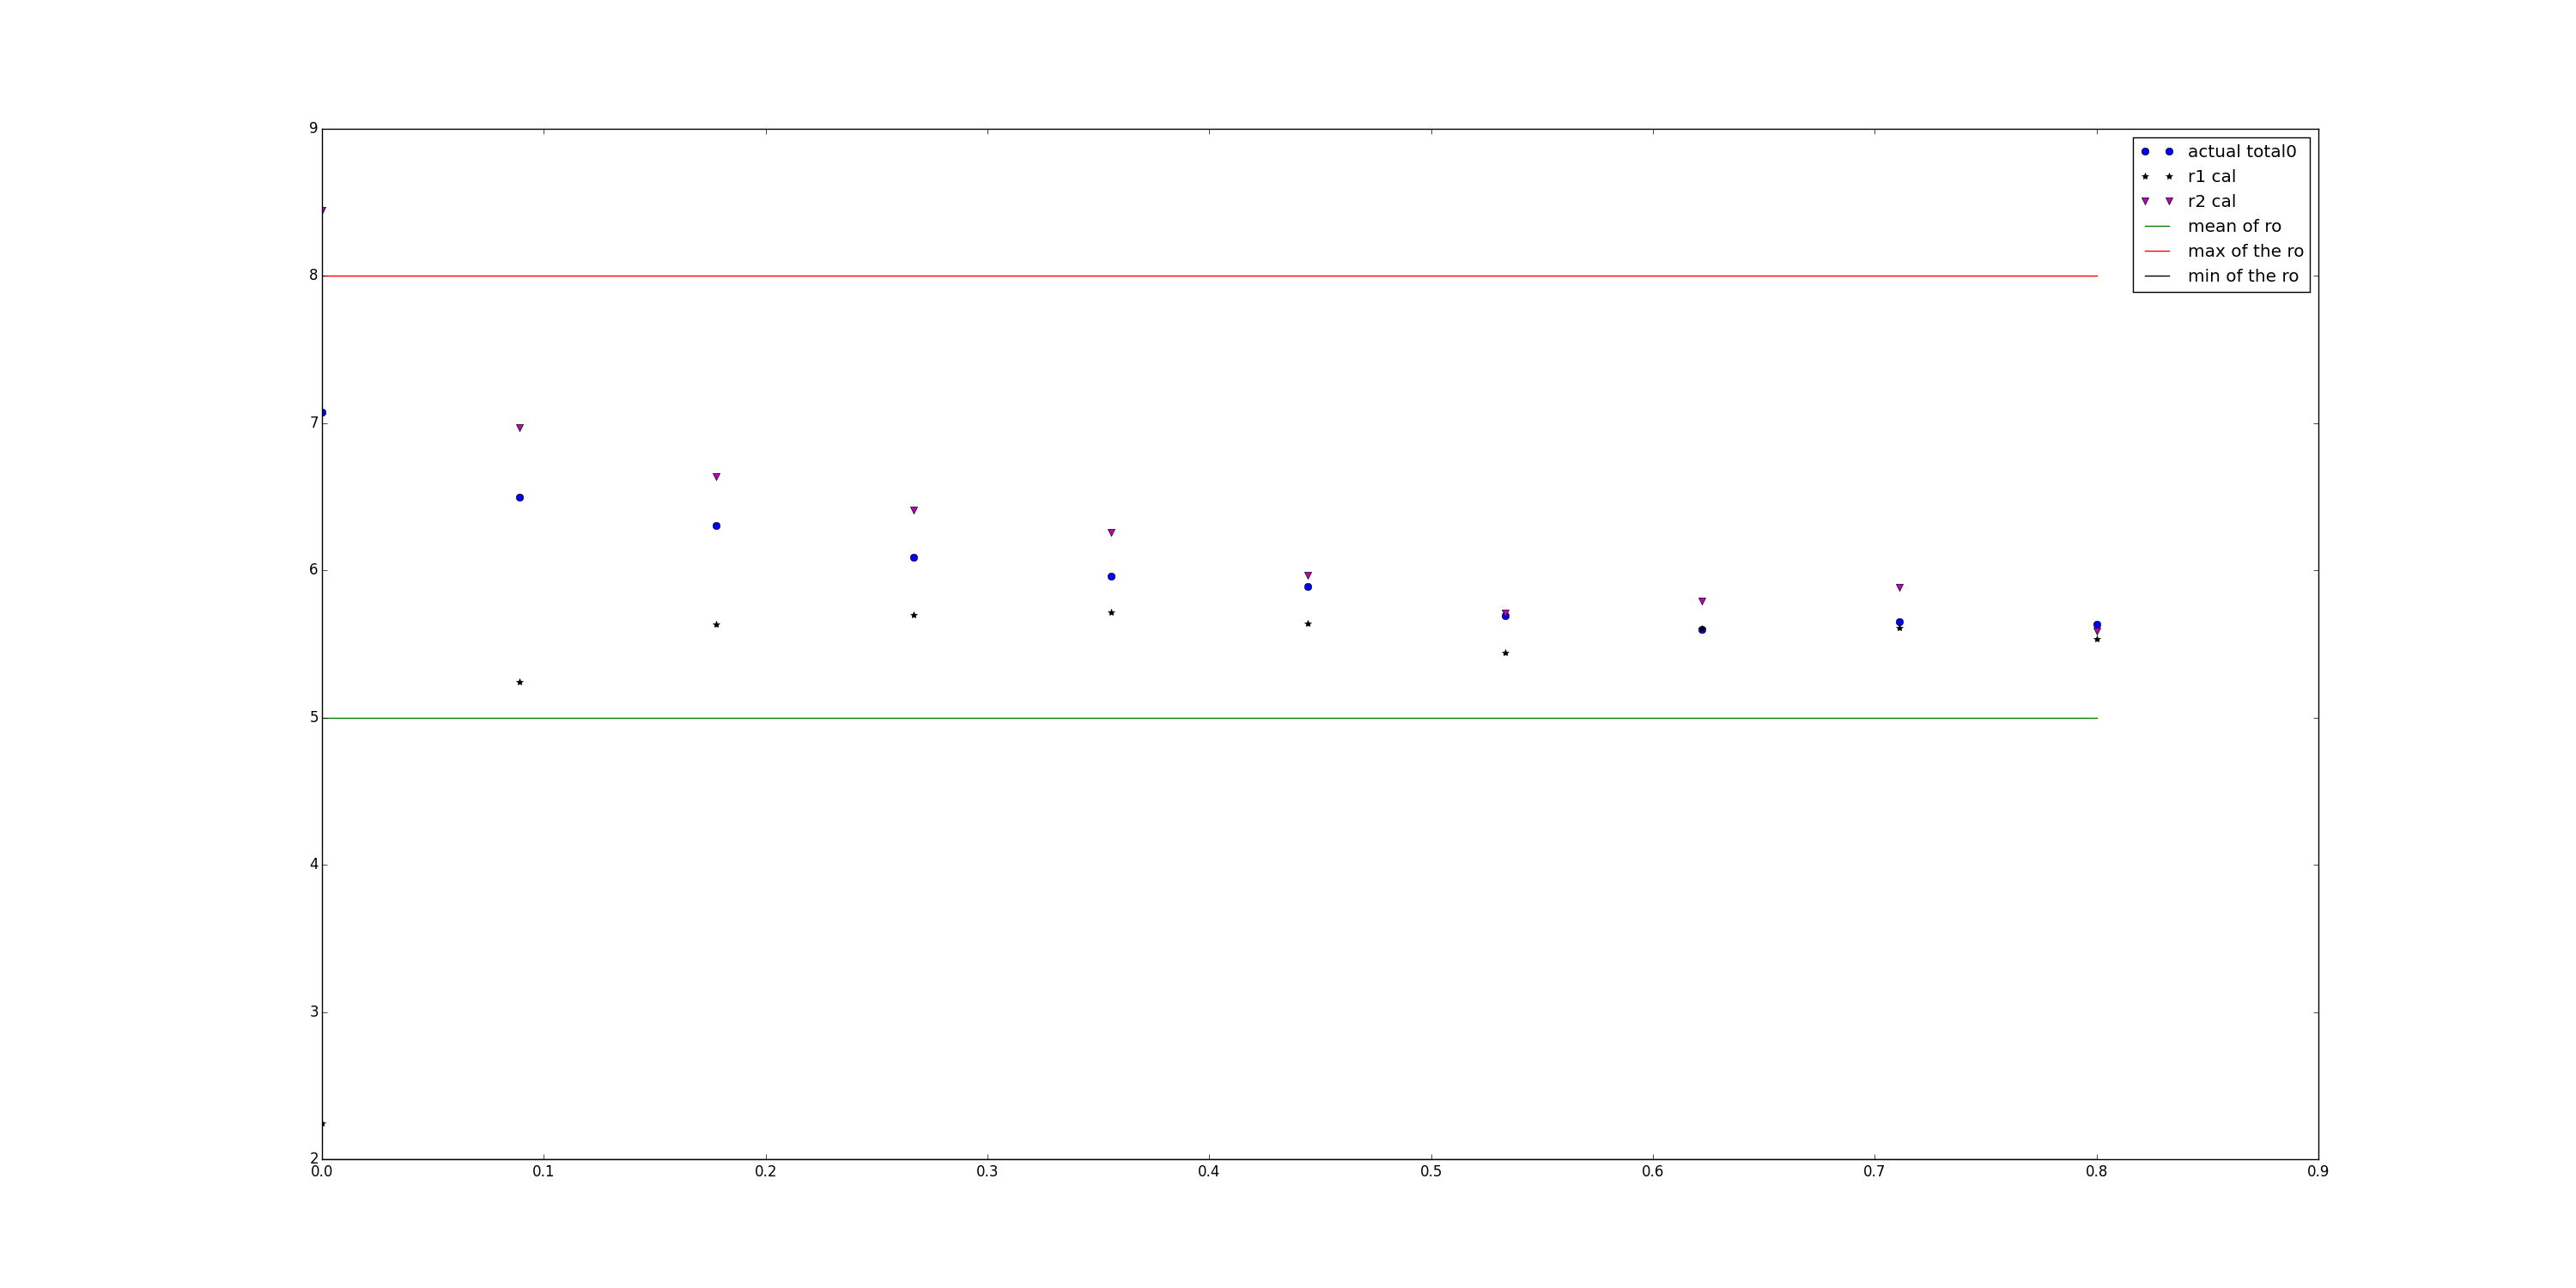
\includegraphics[width=1.1 \textwidth]{result1}
\end{figure}
%Generate a good graph with error bars here
\section{Modelling using SEIR model}
\subsection{Results}
\begin{figure}[H]
  \centering
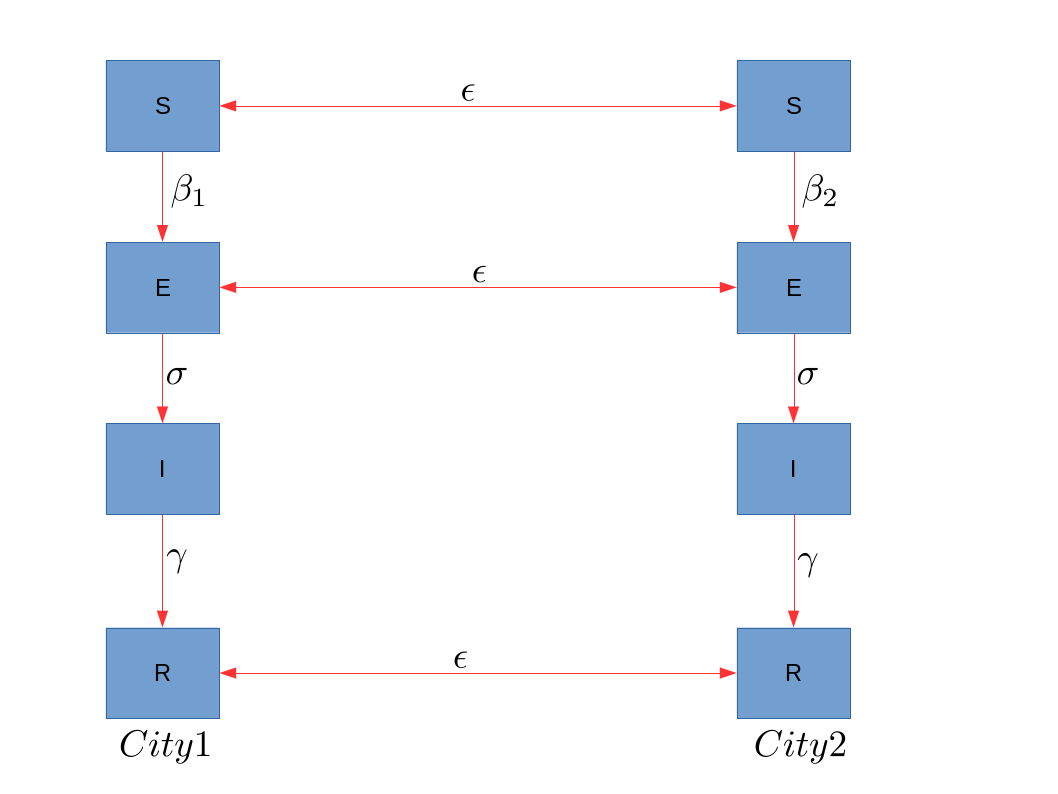
\includegraphics[scale=0.25]{seir_im}
\end{figure}
\textbf{Equations} \newline
$$\frac{dS_{1}}{dt}=\lambda(S_{1}+E_{1}+I_{1}+R_{1}) -\mu  S_{1} - \beta_{1} S_{1}I_{1}  + \epsilon S_{2} -\epsilon S_{1} $$
$$\frac{dE_{1}}{dt}= -\mu  E_{1} + \beta_{1} S_{1}I_{1}  + \epsilon E_{2} -\epsilon E_{1} -\sigma  E_{1} $$
$$\frac{dI_{1}}{dt}= \sigma E_{1} -\gamma I_{1} -\mu I_{1}$$
$$\frac{dR_{1}}{dt}= -\mu  R_{1} +  \epsilon R_{2} -\epsilon R_{1} +\gamma I_{1} $$

$$\frac{dS_{2}}{dt}=\lambda(S_{2}+E_{2}+I_{2}+R_{2}) -\mu  S_{2} - \beta_{2} S_{2}I_{2}  + \epsilon S_{1} -\epsilon S_{2} $$
$$\frac{dE_{2}}{dt}= -\mu  E_{2} + \beta_{2} S_{2}I_{2}  + \epsilon E_{1} -\epsilon E_{2} -\sigma  E_{2} $$
$$\frac{dI_{2}}{dt}= \sigma E_{2} -\gamma I_{2} -\mu I_{2}$$
$$\frac{dR_{2}}{dt}= -\mu  R_{2} +  \epsilon R_{1} -\epsilon R_{2} +\gamma I_{2} $$

Where $\sigma$ denotes the rate of getting infectious from exposed,
all other symbols denotes the same. As you can see we have restricted
the migration of Infected indiciduals between the cites. So the
infection can transfer between the cities only through migration of
exposed individuals. \newline Similar analysis as SIR model was used,
but the relation between $r$ and $R_{0}$ has to be re-derived for this
system.
\subsection{Relation between $r$ and $R_{0}$}
In this model the generation interval distribution
$g(a)=Exp(\frac{1}{\gamma})+Exp(\frac{1}{\sigma})$, where $Exp(\lambda)$
denotes exponential distribution with mean $\lambda$. \newline
Convolution of two expoential distribution with mean
$\frac{1}{\lambda}$ and $\frac{1}{\theta}$ has the following pdf
$$f(x)=\frac{\lambda \theta}{\lambda - \theta}(e^{- \lambda x}-e^{-\theta x})$$
with MGF as
$$M(t)=\frac{\theta \lambda}{(\lambda-t)(\theta-t)}$$.
So in our case $R_{0}$ turns out to be
\begin{equation}
R_{0}=(1+\frac{r}{\gamma})(1+\frac{r}{\sigma})
\end{equation}
Using Eq(5) instead of Eq(4) and similar analysis as SIR model gave us the following result.
\section{Results}
\begin{figure}[H]
  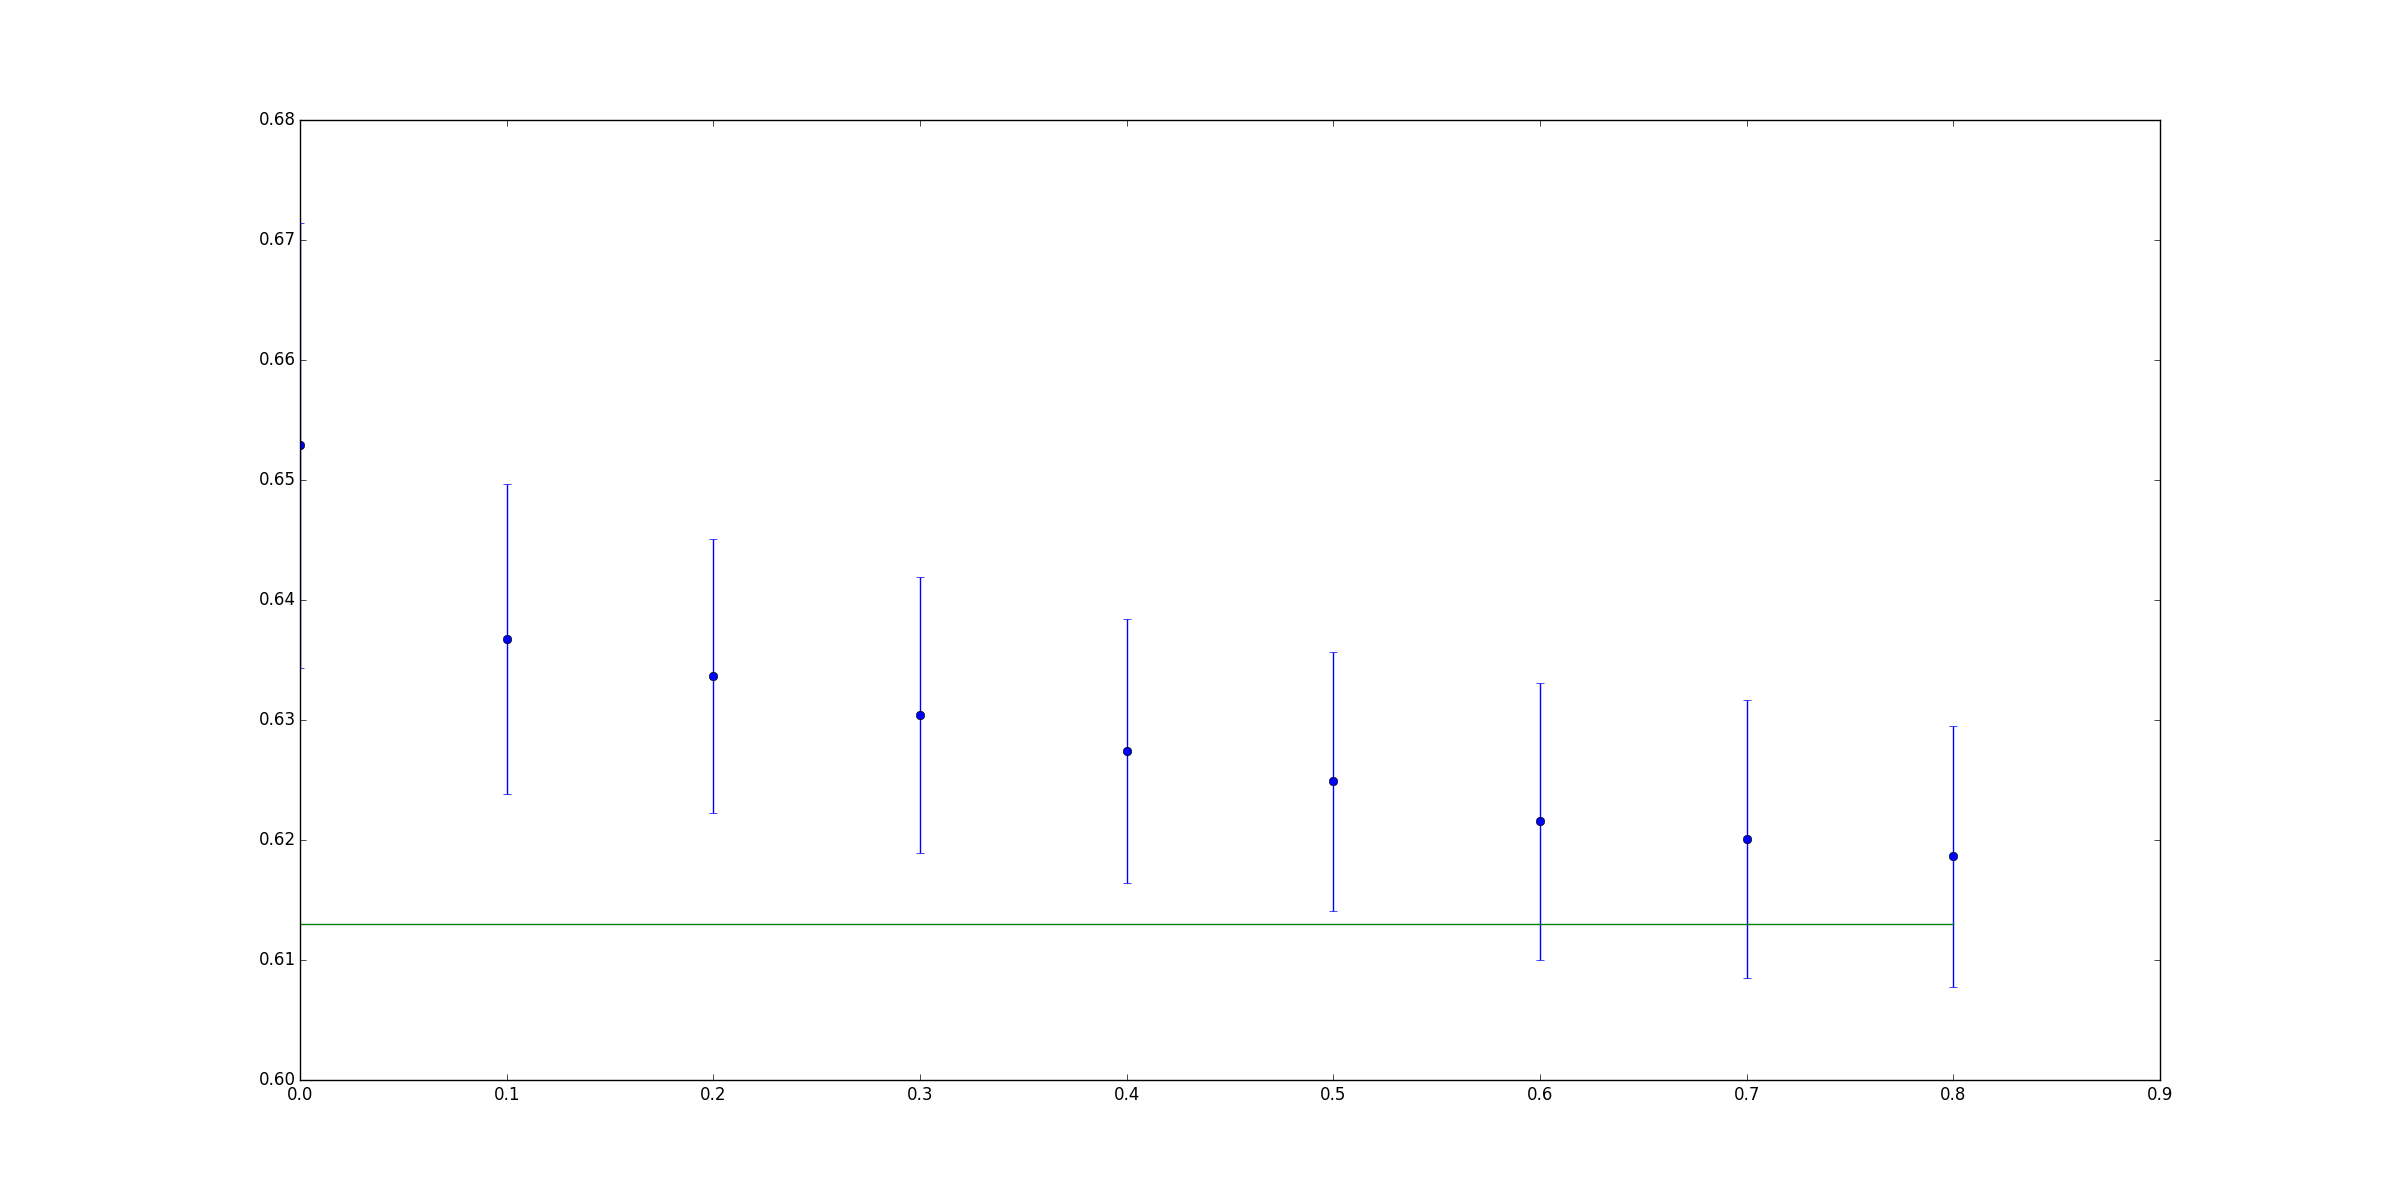
\includegraphics[width=\textwidth]{long_run}
\caption{with infection starting in both the cities}
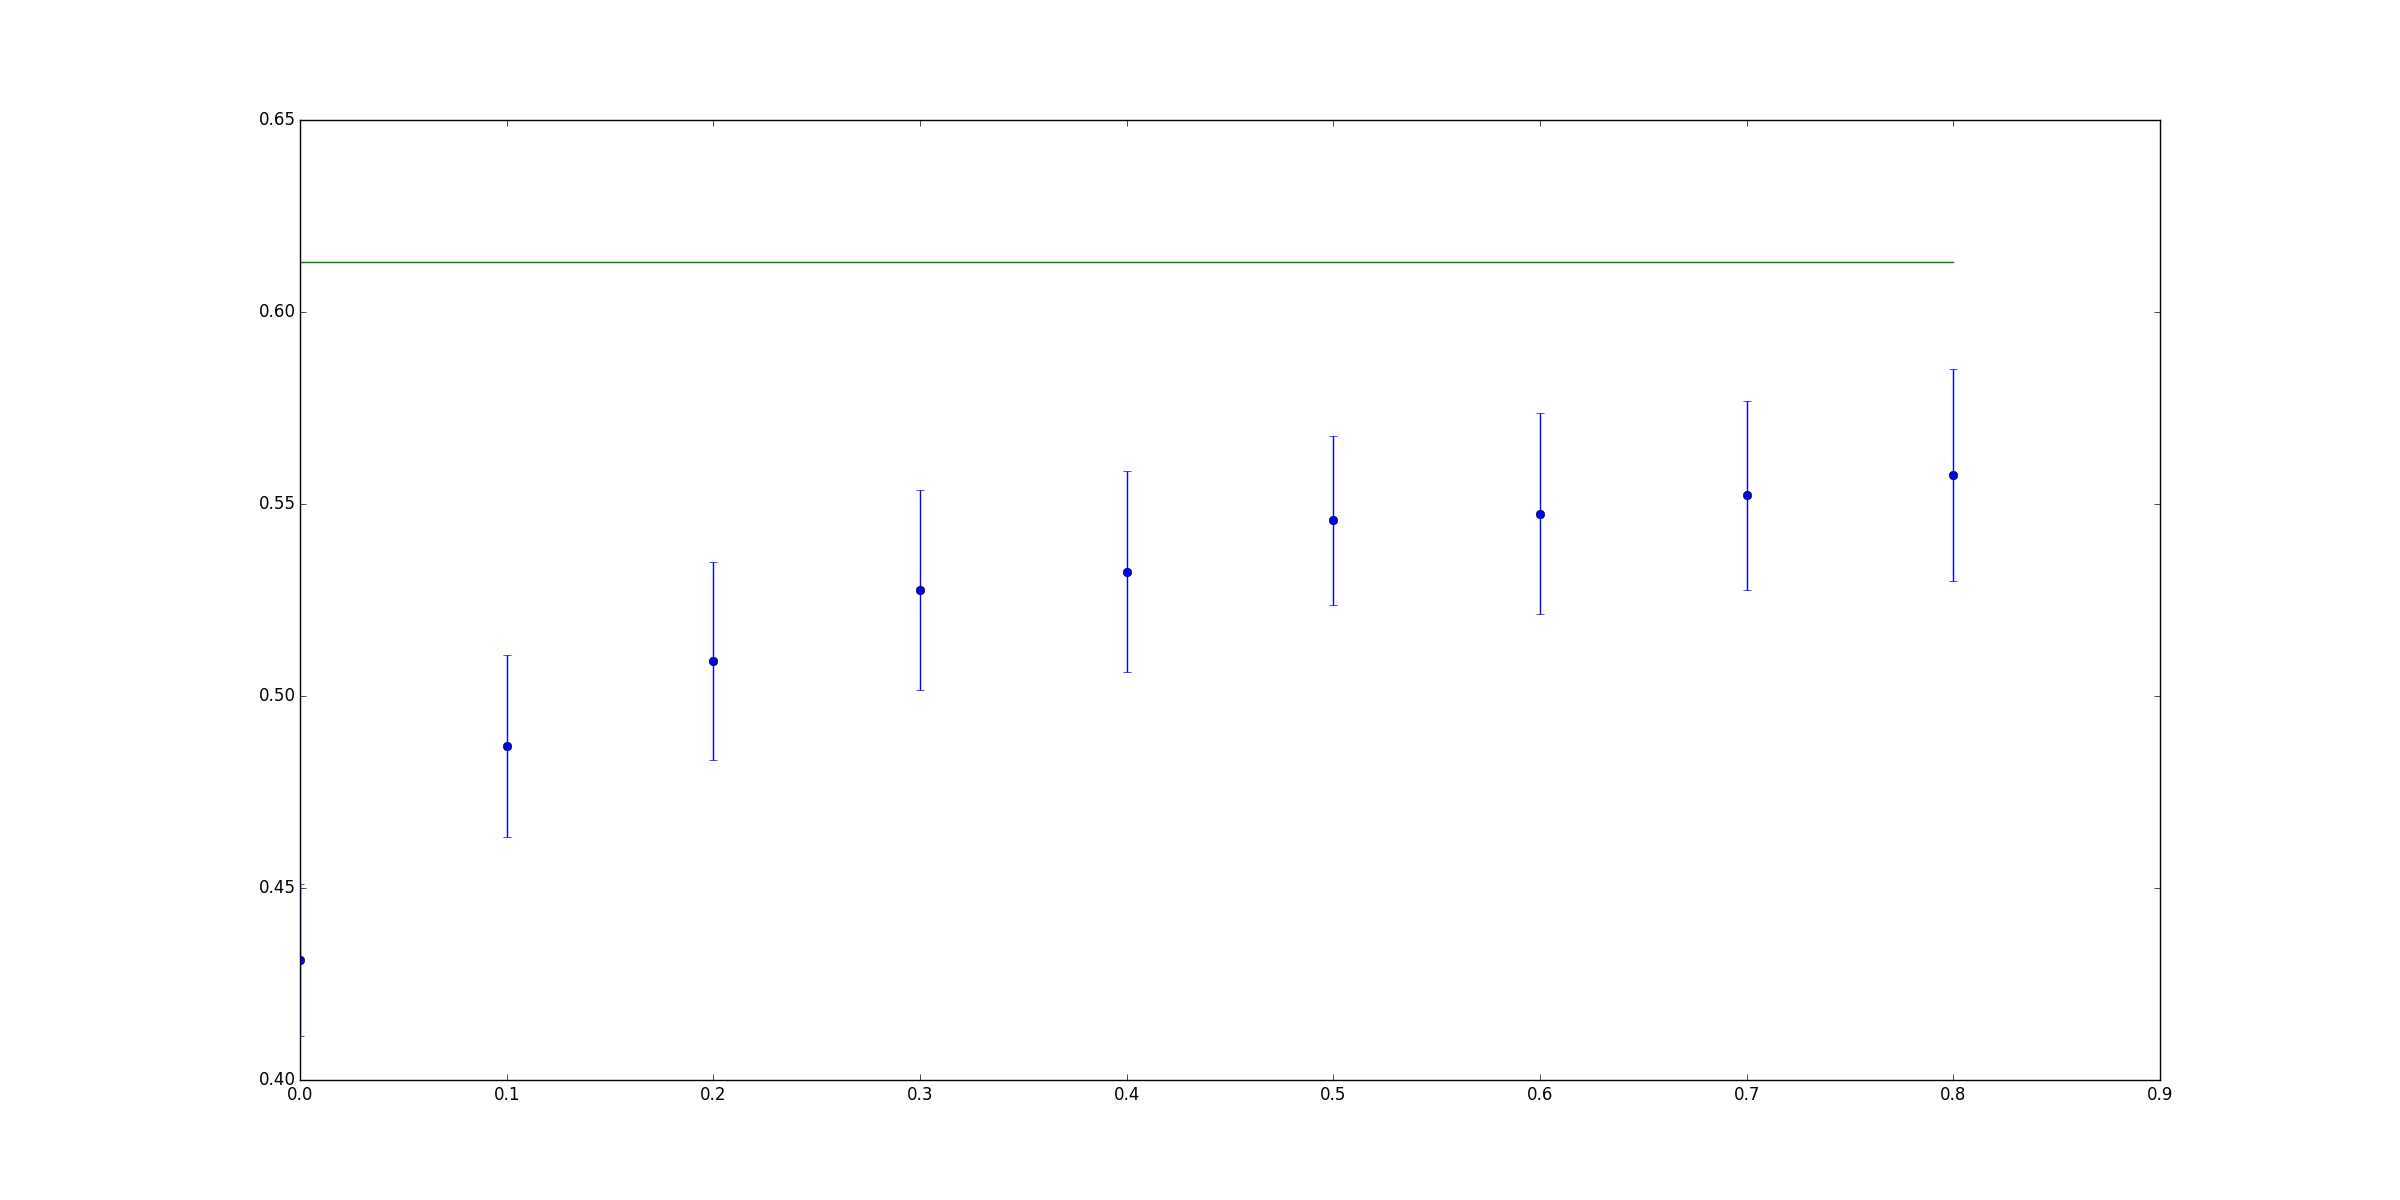
\includegraphics[width=\textwidth]{city1_inf}
\caption{with infection starting at city1}
\end{figure}
\begin{figure}
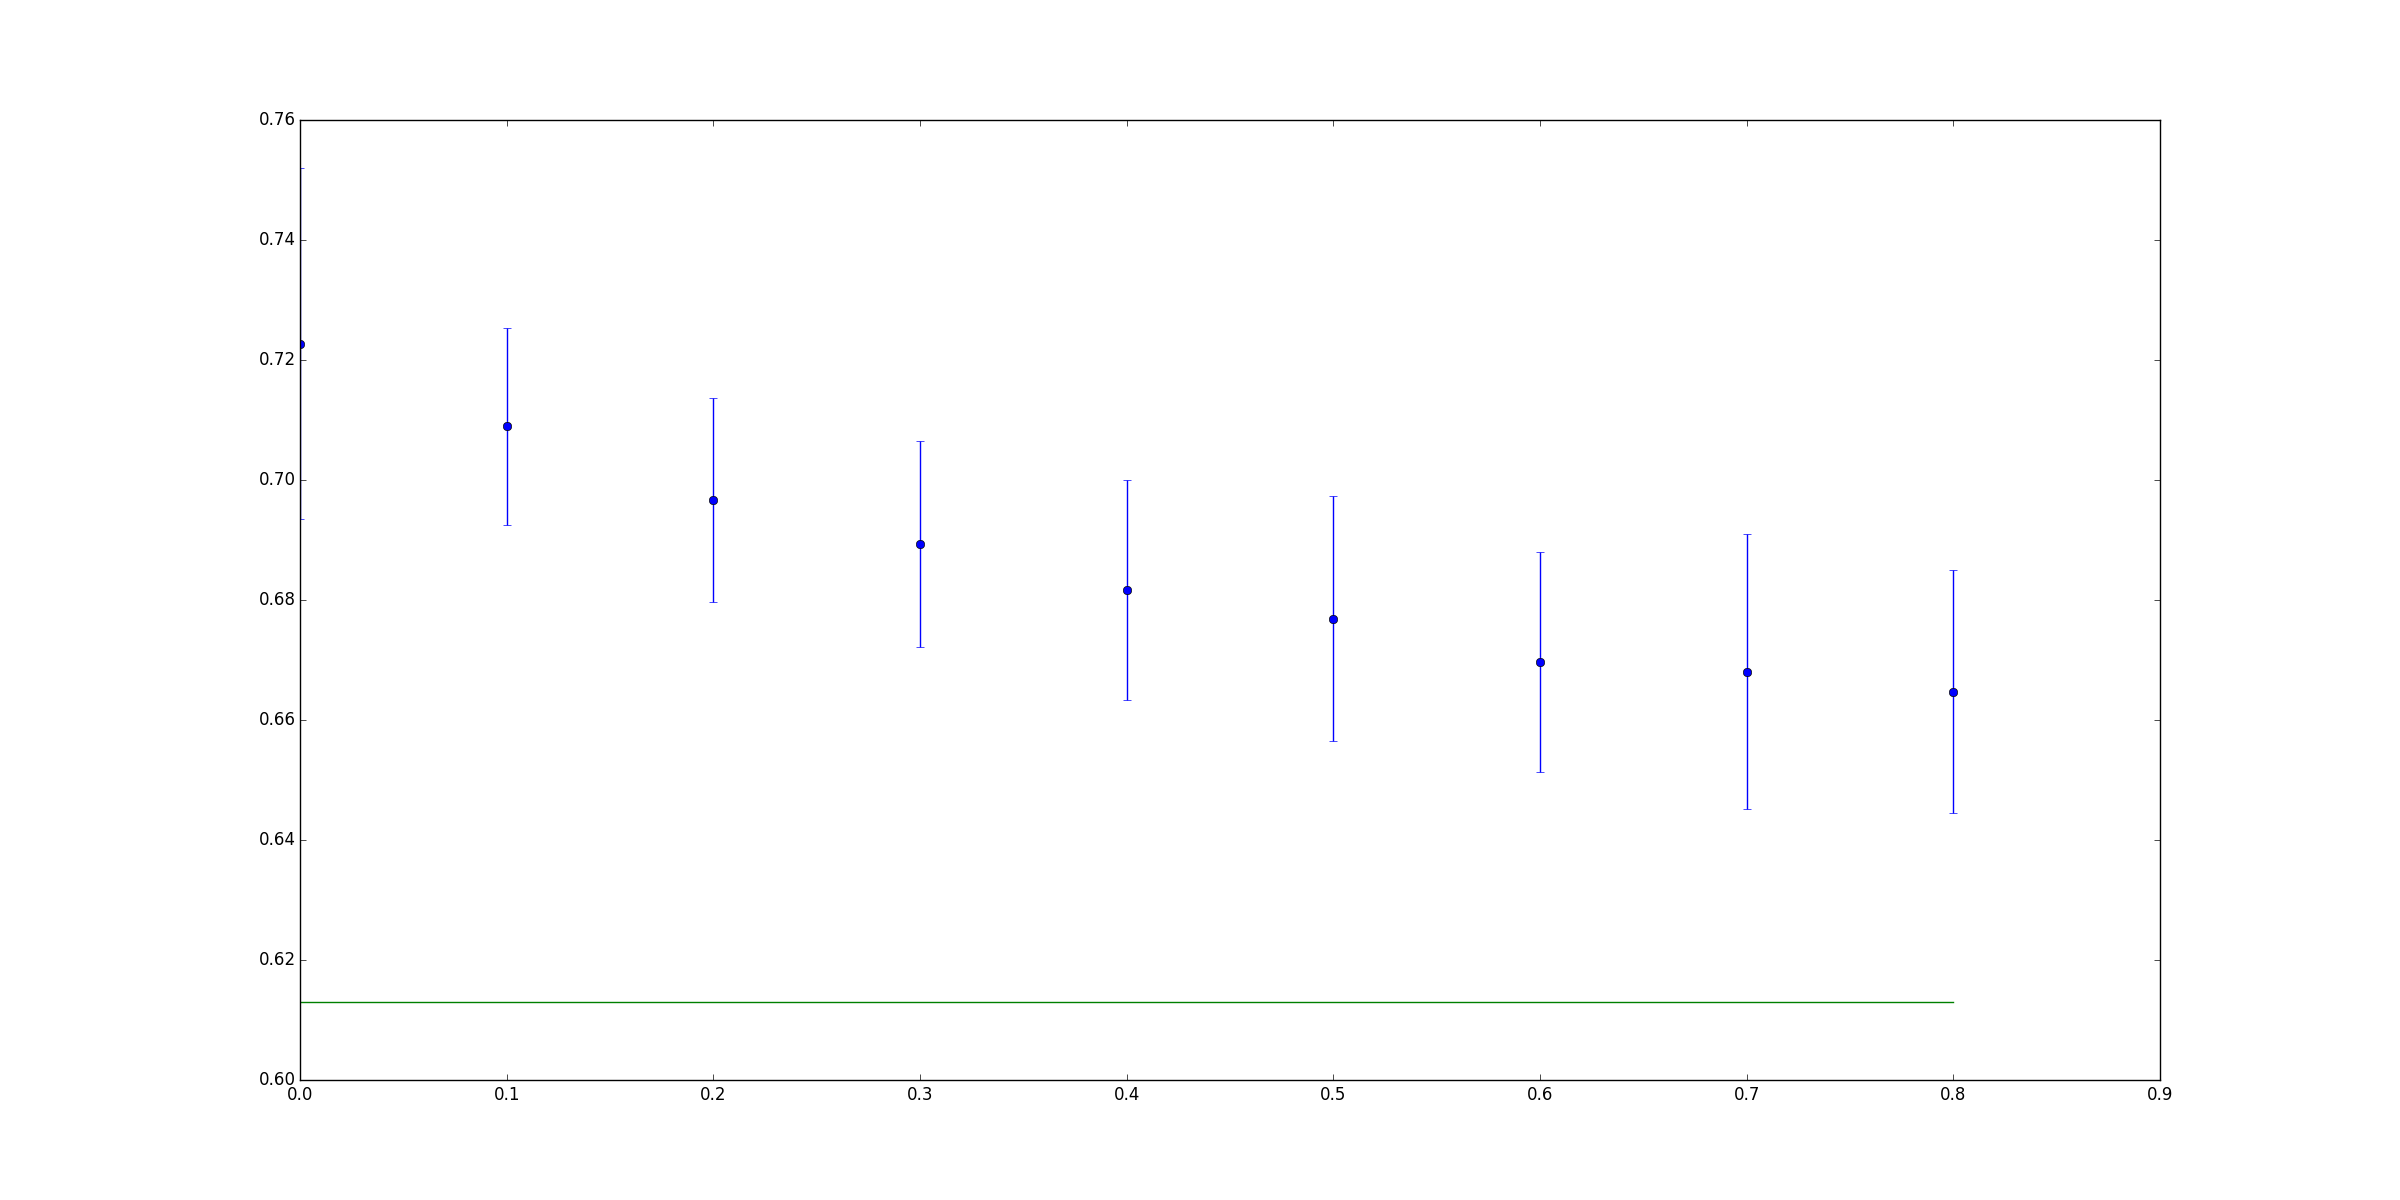
\includegraphics[width=\textwidth]{city2_inf}
\caption{with infection staring at city2}
\end{figure}  
\section{Theoritical derivation}
\subsection{The Next generation operator method}
$R_{0}$ is defined as the spectral radius of the 'next generation
operator'.  To find the next generation operator, we need to first
identify the infected and non-infected compartments. Suppose there are
$n$ compartments of which $m$ are infected. Let $\bar{x}=(x_{1},x_{2},\dots,x_{n})$
where each $x_{i}$ denotes the number of individuals in $i^{th}$ compartment.
Let, $F_{i}(x)$, denote the rate of apperance of new infections in compartment $i$.
$V^{-}_{i}(x)$ be the rate of transfer of individuals into compartment $i$ by all other means and
$V^{+}_{i}(x)$ be the rate of transfer of individuals out of compartment $i$.

$$\frac{dx_{i}}{dt}=F_{i}(x)-V_{i}(x)= f(x_{i})$$  where $V_{i}(x)=V^{+}_{i}(x)-V^{-}_{i}(x)$.

We then construct $\mathcal{F}$ and $\mathcal{V}$ matrices by taking
the partial derivatives of the $F_{i}$ with respect to $x_{i}$ and
similarly for $\mathcal{V}$ by taking partial derivatives of $V_{i}$.
We define $R_{0}$ to be the spectral radius of the $\mathcal{F}\mathcal{V}^{-1}$.\\
\textbf{Spectral radius of square matrix} It is the  largest absolute value of the matrix's eigen value.


\subsection{Assumptions}
\begin{enumerate}
\item If $\bar{x} \geq 0$, then $F_{i},V_{i}^{+}, V_{i}^{-} \geq 0 \forall i$
\item If $\bar{x} = 0$, then $V_{i}^{-} = 0$
\item $F_{i} = 0$ if $i \geq m$
\item If $\bar{x} \in X_{s} $, where $X_{s}$ is set of all Disease Free states. Then $F_{i},V_{i}^{+}=0$
  \item It is assumed that a disease free equilibrium exists and it is a locally asymptotically stable solution of the disease free model.Thus if $x_{0}$ denotes a disease free equilibrium of the system, then if $\mathcal{F}(x)$ is set to zero, then all eigenvalues of $Df(x_{0})$ have negative real parts.
\end{enumerate}
\subsection{SIR model with birth and death}
The following is the derivation of $R_{0}$ for SIR model with birth and death. \\
\textbf{Equations}
$$\frac{dS_{1}}{dt}=\lambda(S_{1}+I_{1}+R_{1}) -\mu  S_{1} - \beta_{1} S_{1}I_{1}  + \epsilon S_{2} -\epsilon S_{1} $$
$$\frac{dI_{1}}{dt}= -\mu  I_{1} + \beta_{1} S_{1}I_{1}  + \epsilon I_{2} -\epsilon I_{1} -\gamma I_{1} $$
$$\frac{dR_{1}}{dt}= -\mu  R_{1} +  \epsilon R_{2} -\epsilon R_{1} +\gamma I_{1} $$
Similarlly for City 2
\begin{itemize}

\item \textbf{For single city in isolation with no transfer rates}\\
  $\epsilon = 0$ , $n=3$ and $m=1$ \\ $F_{i}$ is the rate of
  apperance of infection at compartment $i$, It is enough to consider
  the $I$ compartment, Since only $I$ contributes for the infection.

  $$\frac{dI}{dt}= \beta S I -\gamma I -\mu I$$
  $$F=\beta S I,V= -\gamma I -\mu I$$\
  $$\frac{dF}{dI}=\beta S , \frac{dV}{dI}= -\gamma -\mu$$ 
  at Disease Free equilibrium \textit{$S1=N_{0}$ where $N_{0}$ is the initial number of people} \newline
  $$\frac{dF}{dI} \big|_{DFE}=\beta N_{0} , \frac{dV}{dI} \big|_{DFE}= -\gamma -\mu$$ \\
  $$\mathcal{F}=\frac{dF}{dI} \big|_{DFE},  \mathcal{V}=\frac{dV}{dI} \big|_{DFE}$$ \\
  Since $R_{0}$ equals the spectral radius of $\mathcal{F}\mathcal{V}^{-1}$, We find that
  $$R_{0}=\frac{\beta N}{(\gamma + \mu)}$$

\item \textbf{For two cities with transfer rates} \newline
  $n=6$ and $m=2$ where $I_{1}$ and $I_{2}$ are the two infected compartments.\newline
  $$F_{1} = \beta_{1} S_{1} I_{1} ,  F_{2} = \beta_{2} S_{2} I_{2}$$ 
  $$V_{1}=-\gamma I_{1} -\mu I_{1} -\epsilon I_{1} + \epsilon I{2},   V_{2}=-\gamma I_{2} -\mu I_{2} -\epsilon I_{2} + \epsilon I{1}$$ 
  Now,\\
  \center
    \[
\mathcal{F}=
  \begin{bmatrix}
    \beta_{1} N_{1} & 0 \\
    0 & \beta_{2} N_{2} \\
  \end{bmatrix}
\]
 
\[
\mathcal{V}=
  \begin{bmatrix}
    -\gamma -\mu - \epsilon & \epsilon \\
    \epsilon & -\gamma -\mu -\epsilon \\
  \end{bmatrix}
\]
\end{itemize}
The Eigen values of $\mathcal{F}\mathcal{V}^{-1}$ was calculated using sage,

The spectral radius defined as the absolute value of the largest eigen value turns out to be
$$R_{0}=\frac{X+\sqrt{X^{2}-4\beta_{1}\beta{2}N_{1}N_{2}Y}}{2Y}$$
where $X=(\beta_{1} N_{1}+\beta{2} N_{2})(\epsilon+\mu+\gamma)$ and
$Y=(2 \epsilon \gamma+\gamma^{2}+2 \epsilon \mu+ 2 \mu \gamma+
\mu^{2})$
\subsubsection{Plotting}

\subsection{SEIR Model}
\textbf{Equations} \newline

$$\frac{dS_{1}}{dt}=\lambda(S_{1}+E_{1}+I_{1}+R_{1}) -\mu  S_{1} - \beta_{1} S_{1}I_{1}  + \epsilon S_{2} -\epsilon S_{1} $$
$$\frac{dE_{1}}{dt}= -\mu  E_{1} + \beta_{1} S_{1}I_{1}  + \epsilon E_{2} -\epsilon E_{1} -\sigma  E_{1} $$
$$\frac{dI_{1}}{dt}= \sigma E_{1} -\gamma I_{1} -\mu I_{1}$$
$$\frac{dR_{1}}{dt}= -\mu  R_{1} +  \epsilon R_{2} -\epsilon R_{1} +\gamma I_{1} $$
Similarlly for City 2

\begin{itemize}
\item \textbf{For single city in isolation with no transfer rates}\\
  $\epsilon = 0$ , $n=4$ and $m=2$, $E_{1}$ and $I_{1}$ are considered as infective compartments 
  $$F_{1}= \beta_{1} S_{1} I_{1}, F_{2}=0$$
  $$V_{1}= -\mu E_{1} -\sigma E_{1} , V_{2} = \sigma E_{1} -\gamma
  I_{1} -\mu I_{1}$$ Now, calculating $\mathcal{F}$ and $\mathcal{V}$
  at DFE \textit{$S_{1}=N_{1}$} \newline \center
  \[
\mathcal{F}=
  \begin{bmatrix}
    0 & \beta_{1} N_{1} \\
    0 &  0 \\
  \end{bmatrix}
\]
 
\[
\mathcal{V}=
  \begin{bmatrix}
     -\sigma -\mu & 0  \\
    \sigma & -\gamma -\mu \\
  \end{bmatrix}
\]

The Spectral radius of $\mathcal{F}\mathcal{V}^{-1}$ was calculated using mathematica.
$$R_{0}=\frac{\beta_{1} N_{1} \sigma}{(\gamma + \mu)(\mu +\sigma)}$$

\item \flushleft \textbf{For two cities with transfer rates} \newline
  $n=8$ and $m=4$, $E_{1}$,$I_{1}$,$E_{1}$ and $I_{1}$ are considered as infective compartments.
  $$F_{1}=\beta_{1} S_{1} I_{1}, F_{2}=0$$
  $$F_{3}=\beta_{2} S_{2} I_{2}, F_{4}=0$$
  $$V_{1}=-\mu E_{1}+ \epsilon E_{2} -\epsilon E_{1} -\sigma E_{1}, V_{2}=\sigma E_{1} -\gamma I_{1} -\mu I_{1}$$
  $$V_{3}=-\mu E_{2}+ \epsilon E_{1} -\epsilon E_{2} -\sigma E_{2}, V_{4}=\sigma E_{2} -\gamma I_{2} -\mu I_{2}$$

  Now, calculating $\mathcal{F}$ and $\mathcal{V}$ at DFE \textit{$S_{1}=N_{1}$ and $S_{2}=I_{2}$} \newline

 
 \[
\mathcal{F}=
  \begin{bmatrix}
    0 & \beta_{1} N_{1} & 0 &   0 \\
    0 &  0                & 0 &   0 \\
    0 &  0                & 0 &  \beta_{2} N_{2} \\
    0 &  0                & 0 &   0 \\
  \end{bmatrix}
\]


\[
\mathcal{V}=
  \begin{bmatrix}
     -\sigma -\mu -\epsilon  & 0 & \epsilon  & 0  \\
    \sigma & -\gamma -\mu  & 0 & 0 \\
    \epsilon & 0 & -\sigma -\epsilon -\mu & 0 \\
    0 & 0 & \sigma & -\mu -\gamma
  \end{bmatrix}
\]

\end{itemize}
The Spectral radius of $\mathcal{F}\mathcal{V}^{-1}$ was calculated using sage.
$$R_{0}=\frac{X+\sqrt{X^{2}-4\beta_{1}\beta{2}N_{1}N_{2} \sigma^{2} Y}}{2(\gamma+\mu)Y}$$ where $X=(\beta_{1} N_{1} \sigma+\beta{2} N_{2} \sigma)(\epsilon + \mu + \sigma)$ and $Y=(2 \epsilon \mu+\mu^{2}+2 \epsilon \sigma +2 \mu \sigma +\sigma^{2})$
\subsubsection{Plotting}
\end{document}
